\section{Augmentation of tLDGBAs and Synthesis Method}

We introduce an automaton augmented with binary vectors. The automaton can explicitly represent whether transitions in each accepting set occur at least once, and ensure transitions in each accepting set occur infinitely often.

Let $V = \{ (v_1, \ldots ,v_n)^T\ ;\ v_i \in \{ 0,1 \},\ i \in \{ 1, \ldots ,n \} \}$ be a set of binary-valued vectors, and let $\bm{1}$ and $\bm{0}$ be the $n$-dimentional vectors with all elements 1 and 0, respectively.
In order to augment a tLDBA $B_{\varphi}$, we introduce three functions $visitf:\delta \rightarrow V$, $reset:V \rightarrow V$, and $Max:V\times V \rightarrow V$ as follows.
For any $e \in \delta$, $visitf(e) = (v_1, \ldots ,v_n)^T$, where %$ v_i = 1 $ if $ e \in F_i $ and $ v_i=0 $ otherwise.
\begin{align}
 v_i =
  \left\{
  \begin{aligned}
    1 &   & &\text{if}\ e\in F_i, \\
    0 &   & &\text{otherwise}.
  \end{aligned}
  \right. \nonumber
\end{align}
For any $v \in V$, %$ reset(v) = \bm{0} $ if $ v = \bm{1} $ and $ reset(v) = v $ otherwise.
\begin{align}
  &reset(v) =
  \left\{
  \begin{aligned}
    \bm{0} &   & &\text{if}\  v = \bm{1},\\
    v &   & &\text{otherwise}.
  \end{aligned}
  \right. \nonumber
\end{align}
For any $v,u \in V$, $Max(v,u) = (l_1,\ldots ,l_n)^T$, where $l_i = max\{v_i, u_i\} $ for any $i\in \{1, \ldots ,n\}$.

Intuitively, each vector $v$ represents which accepting sets have been visited. The function $visitf$ returns a binary vector whose $i$-th element is 1 if and only if a transition in the accepting set $F_i$ occurs. The function $reset$ returns the zero vector $\bm{0}$ if at least one transition in each accepting set has occurred after the latest reset. Otherwise, it returns the input vector without change.

\begin{definition}
   For a tLDBA $B_{\varphi} = (X,x_{init},\Sigma,\delta,\mathcal{F})$, its augmented automaton is a tLDBA $\bar{B}_{\varphi}$ = $(\bar{X},\bar{x}_{init},\bar{\Sigma},\bar{\delta},\bar{\mathcal{F}})$, where $\bar{X} = X\times V$, $\bar{x}_{init} = (x_{init}, \bm{0})$, $\bar{\Sigma} = \Sigma$, $\bar{\delta}$ is defined as $\bar{\delta}$ = $\{ ((x,v), \bar{\sigma}, (x^{\prime},v^{\prime})) \in \bar{X} \times \bar{\Sigma} \times \bar{X}\ ;\ (x,\bar{\sigma},x^{\prime}) \in \delta,\ v^{\prime} = reset(Max(v,visitf((x,\bar{\sigma},x^{\prime})))) \}$, and $\mathcal{\bar{F}} = \{ \bar{F_1}, \ldots ,\bar{F_n} \}$ is defined as $\bar{F_i} = \{ ((x,v), \bar{\sigma}, (x^{\prime},v^{\prime})) \in \bar{\delta}\ ;\ (x, \sigma, x^{\prime}) \in F_i,\ v_i = 0,\ visitf((x, \bar{\sigma}, x^{\prime}))_i = 1\}$ for each $ i \in \{1,...,n\}$, where $visitf((x, \bar{\sigma}, x^{\prime}))_i$ is the $i$-th element of $visitf((x, \bar{\sigma}, x^{\prime}))$.
\end{definition}

\begin{definition}
  Given an augmented tLDBA $\bar{B}_{\varphi}$ and an MDP $M$, a tuple $M \otimes \bar{B}_{\varphi} = M^{\otimes} = (S^{\otimes}, A^{\otimes}, {\mathcal A}^{\otimes}, s_{init}^{\otimes}, P^{\otimes}, \delta^{\otimes}, {\mathcal F}^{\otimes})$ is a product MDP, where
  $S^{\otimes} = S \times \bar{X}$ is the finite set of states, $A^{\otimes}=A$ is the finite set of actions, ${\mathcal A}^{\otimes} : S^{\otimes} \rightarrow 2^{A^{\otimes}}$ is the mapping defined as ${\mathcal A}^{\otimes}((s,\bar{x})) = {\mathcal A}(s)$, $s_{init}^{\otimes} = (s_{init},\bar{x}_{init})$ is the initial states, $P^{\otimes} : S^{\otimes} \times S^{\otimes} \times A^{\otimes} \rightarrow [0,1]$ is the transition probability defined as
  \begin{align}
    P^{\otimes}(s^{\otimes \prime} | s^{\otimes}, a) =
    \left\{
    \begin{aligned}
      &P(s^{\prime} | s, a) &   &\text{if}\  (\bar{x}, L((s,a,s^{\prime})), \bar{x}^{\prime}) \in \bar{\delta},\\
      &0 &   &\text{otherwise} ,
    \end{aligned}
    \right. \nonumber
  \end{align}
  $\delta^{\otimes} = \{ (s^{\otimes}, a, s^{\otimes \prime}) \in S^{\otimes} \times A^{\otimes} \times S^{\otimes} ; P^{\otimes}(s^{\otimes \prime} | s^{\otimes}, a) > 0 \}$ is the set of transitions, and ${\mathcal F}^{\otimes} = \{ \bar{F}^{\otimes}_1, \ldots ,\bar{F}^{\otimes}_n \}$ is the acceptance condition, where $\bar{F}^{\otimes}_i = \{ ((s,\bar{x}), a, (s^{\prime}, \bar{x}^{\prime})) \in \delta^{\otimes}\ ;\ (\bar{x}, L(s,a,s^{\prime}), \bar{x}^{\prime}) \in \bar{F}_i \}$ for each $ i \in \{ 1, \ldots ,n \}$.
\end{definition}

\begin{definition}
  The reward function $\mathcal{R} :S^{\otimes} \times A^{\otimes} \times S^{\otimes} \rightarrow {\mathbb R}_{\geq 0}$ is defined as
  \begin{align}
    \mathcal{R}(s^{\otimes}, a, s^{\otimes \prime}) =
    \left\{
    \begin{aligned}
      &r_p \  \text{if}\ \exists i \in \! \{ 1, \ldots ,n \},\ (s^{\otimes}, a, s^{\otimes \prime}) \in \bar{F}^{\otimes}_i \!,\\
      &0   \ \ \text{otherwise},
    \end{aligned}
    \right. \nonumber
  \end{align}
  where $r_p$ is a positive value.
\end{definition}

%The reward assignments are based on the acceptance conditions of the product MDP.
Under the product MDP $M^{\otimes}$ and the reward function $\mathcal{R}$, which is based on the acceptance condition of $ M^\otimes $, we show that if there exists a positional policy $\pi$ satisfying the LTL specification $\varphi$, maximizing the expected discounted reward produces a policy satisfying $\varphi$.

For a Markov chain $MC^{\otimes}_{\pi}$ induced by a product MDP $M^{\otimes}$ with a positional policy $\pi$, let $S^{\otimes}_{\pi}= T^{\otimes}_{\pi} \sqcup R^{\otimes 1}_{\pi} \sqcup \ldots \sqcup R^{\otimes h}_{\pi}$ be the set of states in $MC^{\otimes}_{\pi}$, where $T^{\otimes}_{\pi}$ is the set of transient states and $R^{\otimes i}_{\pi}$ is the recurrent class for each $i \in \{ 1, \ldots ,h \}$, and let $R(MC^{\otimes}_{\pi})$ be the set of all recurrent classes in $MC^{\otimes}_{\pi}$. Let $\delta^{\otimes}_{\pi,i}$ be the set of transtions in a recurrent class $R^{\otimes i}_{\pi}$, namely $\delta^{\otimes}_{\pi,i} = \{ (s^{\otimes},a,s^{\otimes \prime}) \in \delta^{\otimes} ; s^{\otimes} \in R^{\otimes i}_{\pi},\ P^{\otimes}(s^{\otimes \prime}|s^{\otimes},a) > 0 \}$, and let $P^{\otimes}_{\pi}$ : $S^{\otimes}_{\pi} \times S^{\otimes}_{\pi} \rightarrow [0,1]$ be the transition probability under $\pi$.

\begin{lemma}
  For any policy $\pi$ and any recurrent class $R^{\otimes i}_{\pi}$ in the Markov chain $MC^{\otimes}_{\pi}$,
  $MC^{\otimes}_{\pi}$ satisfies one of the following conditions.
  \vspace{2mm}
  \begin{enumerate}
    \item $\delta^{\otimes}_{\pi,i} \cap \bar{F}^{\otimes}_j \neq \emptyset\ $, $ \forall j \in \{ 1, \ldots ,n \}$,
    \item $\delta^{\otimes}_{\pi,i} \cap \bar{F}^{\otimes}_j = \emptyset\ $, $ \forall j \in \{ 1, \ldots ,n \}$.
  \end{enumerate}
  \label{lemma3-1}
\end{lemma}

Lemma \ref{lemma3-1} implies that for an LTL formula $\varphi$ if a path $\rho$ under a policy $\pi$ does not satisfy $\varphi$, then the agent obtains no reward in recurrent classes; otherwise there exists at least one recurrent class where the agent obtains rewards infinitely often.

\begin{theorem}
  Let $M^{\otimes}$ be the product MDP corresponding to an MDP $M$ and an LTL formula $\varphi$. If there exists a positional policy satisfying $\varphi$, then there exists a discount factor $\gamma^{\ast}$ such that any algorithm that maximizes the expected reward with $\gamma > \gamma^{\ast}$ will find a positional policy satisfying $\varphi$.
  \label{theorem3-1}
\end{theorem}

%\begin{theorem}
%  Let $M^{\otimes}$ be the product MDP corresponding to an MDP $M$ and an LTL formula $\varphi$. If there exists a positional policy $\pi$ such that $Pr^M_{\pi}(\rho_{init} \models \varphi) = 1$, then there exists a discount factor $\gamma^{\ast}$ such that any algorithm that maximizes the expected reward with $\gamma > \gamma^{\ast}$ will find a positional policy $\pi^{\prime}$ such that $Pr^M_{\pi^{\prime}}(\rho_{init} \models \varphi) = 1$.
%  \label{theorem3-2}
%\end{theorem}

We show the overall procedure of our proposed method in Algorithm \ref{syn_pol}. We employ Q-learning in Algorithm \ref{syn_pol}, but any algorithms maximizing the expected discounted reward can be applied to our proposed method.
\begin{algorithm}
 \caption{RL-based synthesis of control policy on the MDP with the augmented tLDBA.}
 \begin{algorithmic}[1]
 \renewcommand{\algorithmicrequire}{\textbf{Input:}}
 \renewcommand{\algorithmicensure}{\textbf{Output:}}
 \REQUIRE LTL formula $\varphi$ and MDP $M$
 \ENSURE  Optimal policy $\pi^{\ast}$ on the product MDP $M^{\otimes}$
 \STATE Translate $\varphi$ into tLDBA $B_{\varphi}$.
  \STATE Augment $B_{\varphi}$ to $\bar{B}_{\varphi}$.
  \STATE Construct the product MDP $M^{\otimes}$ of $M$ and $\bar{B}_{\varphi}$.
  \STATE Initialize $Q:S^{\otimes} \times A^{\otimes} \rightarrow \mathbb{R}_{\geq 0}$.
  \STATE Initialize episode length $T$.
  \WHILE {$Q$ is not converged}
  \STATE $s^{\otimes} \leftarrow (s_{init},(x_{init},\bm{0}))$.
  \FOR {$t = 1$ to $T$}
  \STATE Choose the action $a$ by a policy $\pi$.
  \STATE Observe the next state $s^{\otimes \prime}$.
  \STATE $Q(s^{\otimes},a) \leftarrow Q(s^{\otimes},a) + \alpha \{ \mathcal{R}(s^{\otimes},a,s^{\otimes \prime}) + \gamma \max_{a^{\prime}}Q(s^{\otimes \prime},a^{\prime}) - Q(s^{\otimes},a) \}$
  \STATE $s^{\otimes} \leftarrow s^{\otimes \prime}$
  \ENDFOR
  \ENDWHILE
 \end{algorithmic}
 \label{syn_pol}
\end{algorithm}

\section{Example}

\begin{figure}[bp]
    \centering
    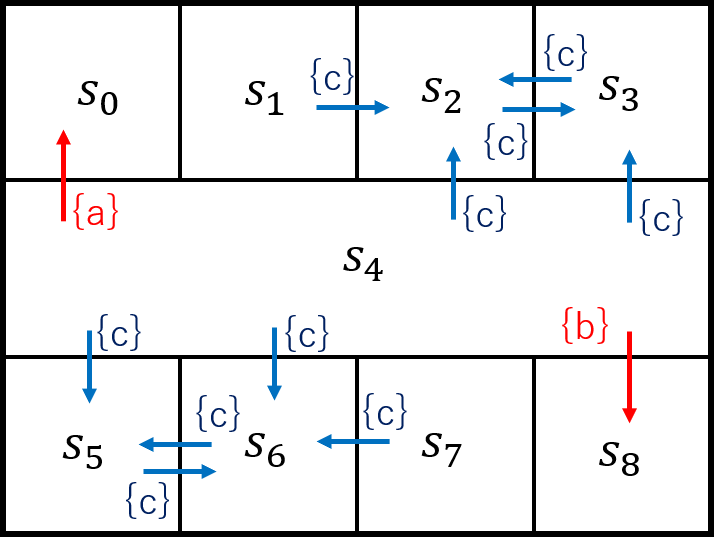
\includegraphics[bb=0 0 377 290,height=3.5cm,width=5cm]{MDP_corridor.png}
%    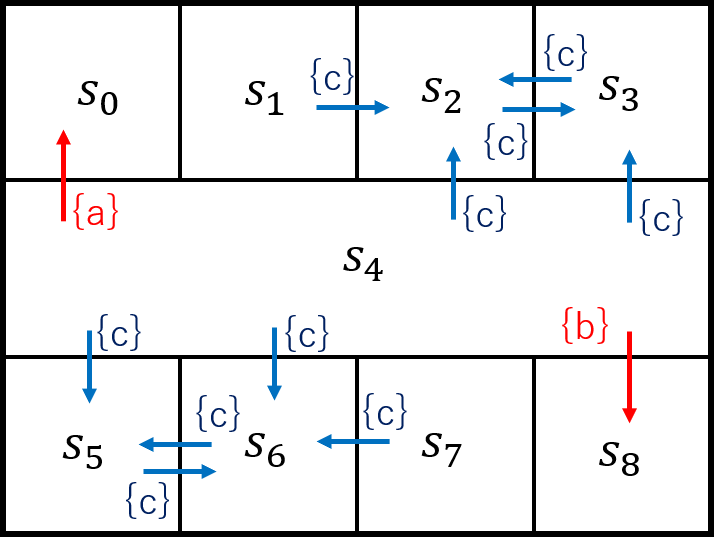
\includegraphics[height=4cm, width=6cm]{MDP_corridor.png}
    \caption{The environment consisting of eight rooms and one corridor. Red arcs are the transitions that we want to occur infinitely often, while blue arcs are the transitions that we never want to occur. $s_7$ is the initial state.}
    \label{Grid1}
\end{figure}

\begin{comment}
\begin{figure}[htbp]
   \centering
   \vspace{2mm}
%   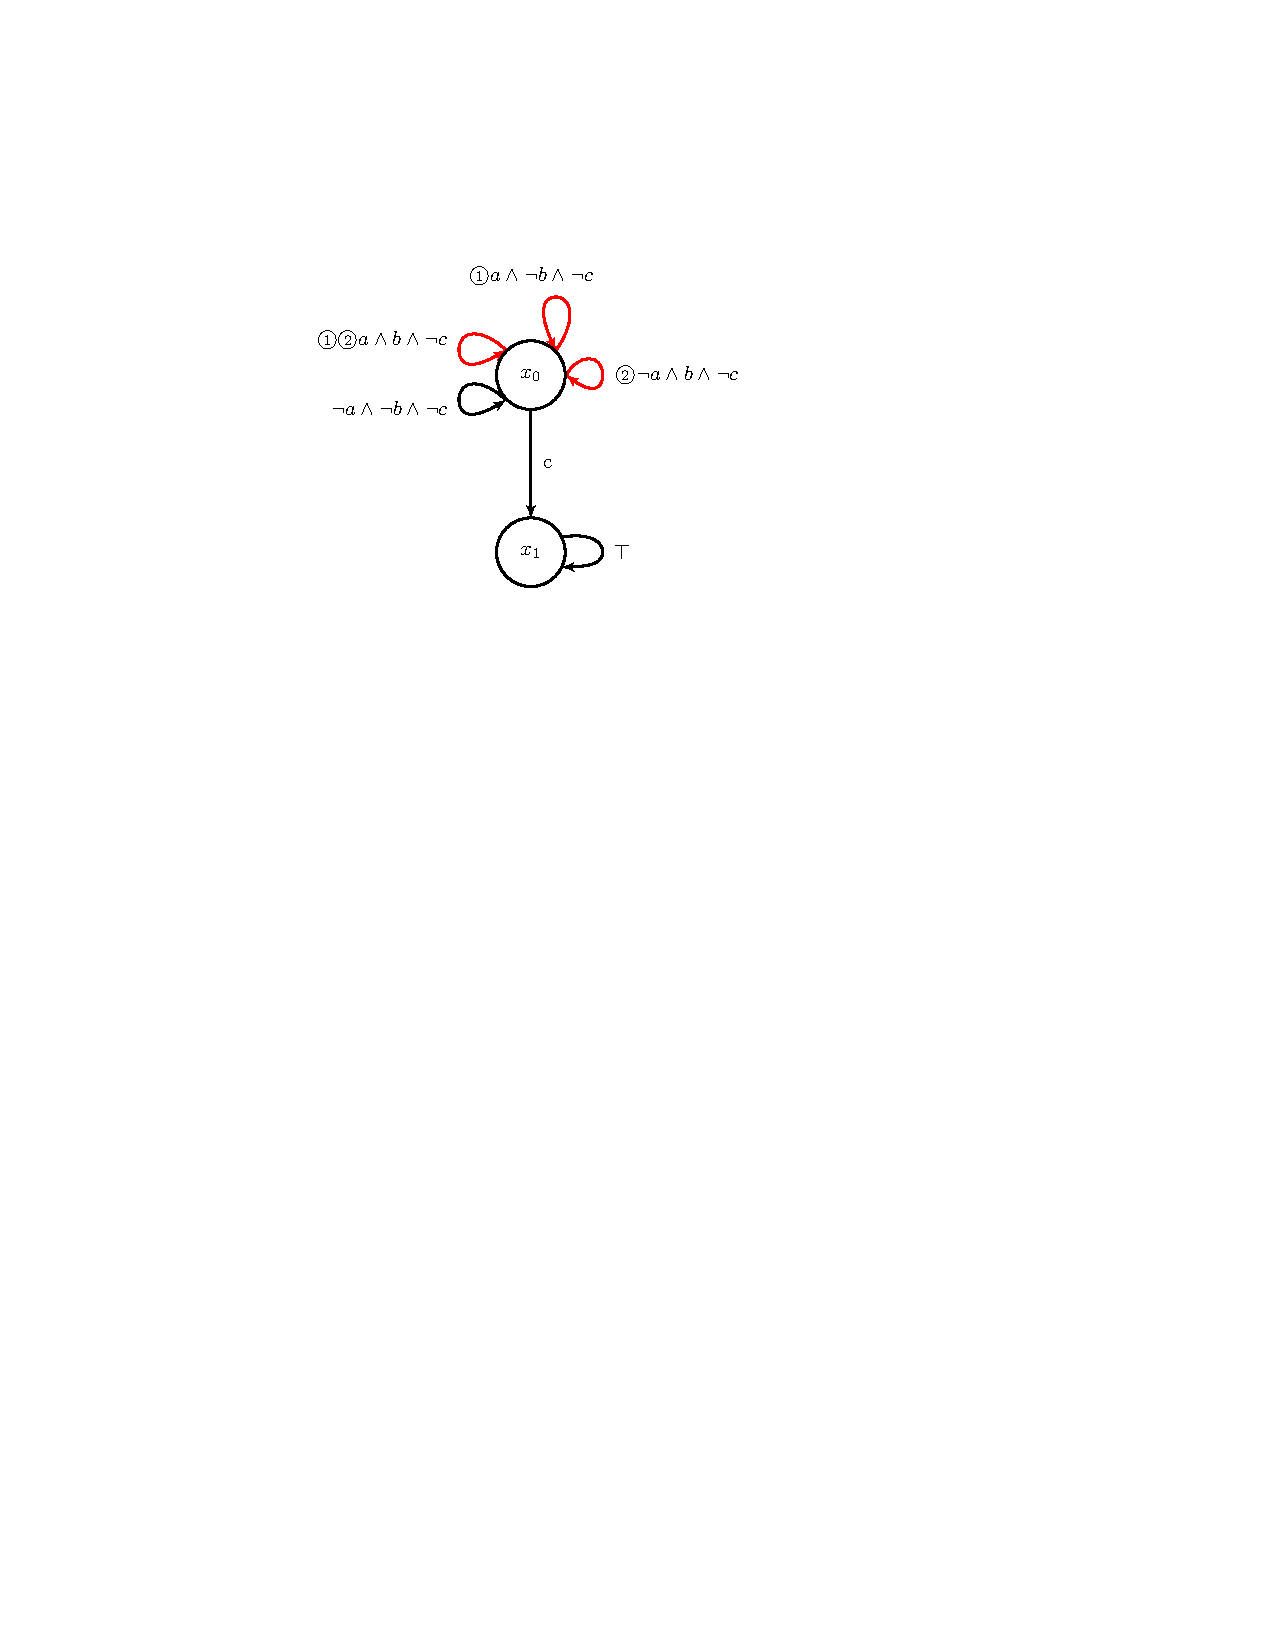
\includegraphics[bb=140 498 368 682,width=5cm]{automaton1.pdf}
   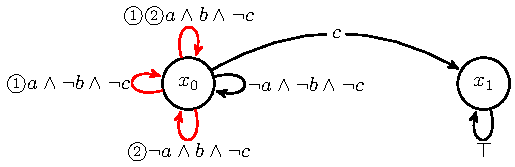
\includegraphics[bb=0 0 247 80,scale=0.65]{ldgba_original.pdf}
   \caption{The tLDGBA recognizing the LTL formula $\text{{\bf GF}}a \wedge \text{{\bf GF}}b \wedge \text{{\bf G}}\neg c$, where the initial state is $x_0$. Red arcs are accepting transitions that are numbered in accordance with the accepting sets they belong to.}
   % e.g., \textcircled{\scriptsize 1}$a \land \neg b \land \neg c$ means the transition labeled by it belongs to the accepting set $F_1$.}
   \label{automaton}
\end{figure}

\begin{figure}[htbp]
   \centering
%   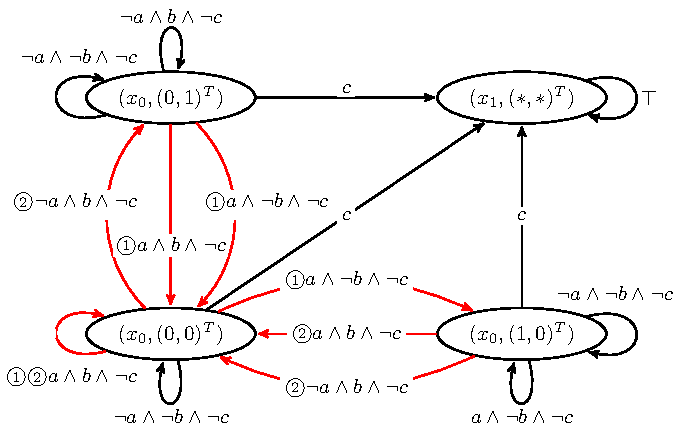
\includegraphics[bb=0 0 374 207,height=4cm, width=7cm]{ldgba.pdf}
   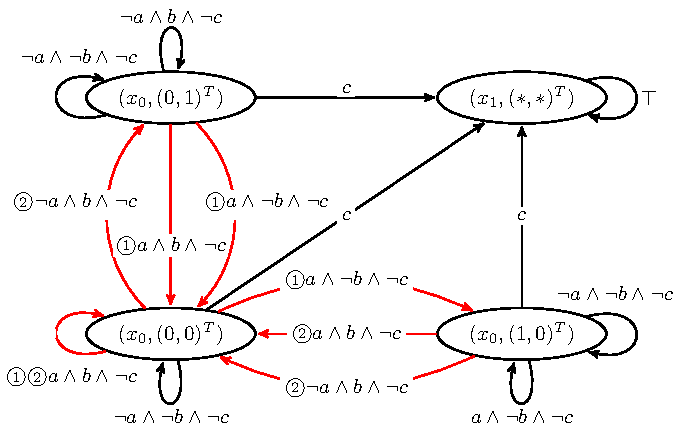
\includegraphics[bb=0 0 374 207,scale=0.6]{ldgba.pdf}
   \caption{The augmented automaton for the tLDGBA in Fig.~\ref{automaton} recognizing the LTL formula $\text{{\bf GF}}a \wedge \text{{\bf GF}}b \wedge \text{{\bf G}}\neg c$, where the initial state is $(x_0, (0,0)^T )$. Red arcs are accepting transitions that are numbered in accordance with the accepting sets they belong to. All states corresponding to $x_1$ are merged into $(x_1, (*,*)^T )$.}
   \label{automaton_aug}
\end{figure}
\end{comment}

In this section, we compare our proposed method with the method in \cite{HAK2019,HKAKPL2019} and the method using tLDBA. In the method using tLDBA, the reward function is defined like Def.\ \ref{def10}, namely it is based on the one accepting set of the corresponding product MDP.
We consider a path planning problem of a robot in an environment consisting of eight rooms and one corridor as shown in Fig.\ \ref{Grid1}. The state $s_7$ is the initial state and the action space is specified with $\mathcal{A}(s) = \{ Right,\ Left,\ Up,\ Down \}$ for any state $s \neq s_4$ and $\mathcal{A}(s_4) = \{ to\_s_0,\ to\_s_1,\ to\_s_2,$ $\ to\_s_3,\ to\_s_5,\ to\_s_6,\ to\_s_7,\ to\_s_8 \}$, where $to\_s_i$ means attempting to go to the state $s_i$ for $i \in \{0,\ 1,\ 2,\ 3,\ 5,\ 6,\ 7,\ 8 \}$. The robot moves in the intended direction with probability 0.9 and it stays in the same state with probability 0.1 if it is in the state $s_4$. In the states other than $s_4$, it moves in the intended direction with probability 0.9 and it moves in the opposite direction to that it intended to go with probability 0.1. If the robot tries to go to outside the environment, it stays in the same state. The labeling function is as follows.
\begin{align*}
      & L((s, a, s^{\prime})) =
      \left\{
      \begin{aligned}
        & \{ c \} &  & \text{if }s^{\prime} = s_i,\ i \in \{ 2,3,5,6 \}, \nonumber \\
        & \{ a \} &  & \text{if }(s,a,s^{\prime})=(s_4,to\_s_0,s_0), \nonumber \\
        & \{ b \} &  & \text{if }(s,a,s^{\prime})=(s_4,to\_s_8, s_8), \nonumber \\
        & \emptyset &  & \text{otherwise}.
      \end{aligned}
      \right.
    \end{align*}

In the example, the robot tries to take two transitions that we want to occur infinitely often, represented by arcs labeled by \{$a$\} and \{$b$\}, while avoiding unsafe transitions represented by the arcs labeled by \{{\it c}\}. This is formally specified by the following LTL formula.
\begin{align*}
  \varphi = \text{{\bf GF}}a \wedge \text{{\bf GF}}b \wedge \text{{\bf G}}\neg c.
\end{align*}
The above LTL formula requires the robot to keep on entering the two rooms $s_0$ and $s_8$ from the corridor $s_4$ regardless of the order of entries, while avoiding entering the four rooms $s_2$, $s_3$, $s_5$, and $s_6$. They have two accepting sets.

%We use Owl \cite{Owl} to obtain the tLDBA corresponding to the LTL formula.
The tLDBA $B_{\varphi} = (X, x_{init},\Sigma,\delta,\mathcal{F})$ and its augmented automaton $\bar{B}_{\varphi} = (\bar{X},\bar{x}_{init},\bar{\Sigma},\bar{\delta},\bar{\mathcal{F}})$ are shown in Figs.\ \ref{automaton} and \ref{automaton_aug}, respectively.

For the three methods, we use Q-learning\footnote{We employ Q-learning here but any algorithm that maximizes the discounted expected reward can be applied to our proposed method.} with $\varepsilon$-greedy policy and gradually reduce $\varepsilon$ to 0 to learn an optimal policy asymptotically.
We set the positive reward $r_p = 2$, the epsilon greedy parameter $ \varepsilon = \frac{0.95}{n_t(s^{\otimes})}$, where $n_t(s^{\otimes})$ is the number of visits to state $s^{\otimes}$ within $t$ time steps \cite{Singh1998}, and the discount factor $\gamma = 0.95$. The learning rate $\alpha$ varies in accordance with {\it the Robbins-Monro condition}. We train the agent in 10000 iterations and 1000 episodes for 20 learning sessions.

 In \cite{HAK2019,HKAKPL2019}, the accepting frontier function is proposed, which is $Acc : X \times 2^X \rightarrow 2^X $ where $X$ is the set of states of the state-based LDBA. Under initializing a set of states $ \mathbb{F} $ with the union of the all accepting sets of the state-based LDBA, the function receives the state $x$ after each transition and the set $\mathbb{F}$. If $x$ is in $\mathbb{F}$, then $Acc$ removes the accepting sets containing $x$ from $\mathbb{F}$. For the product MDP of an MDP $M$ and a state-based LDBA $B_{\varphi}$, the reward function depends on the removed states of $B_{\varphi}$.
 We use the tLDGBA shown in Fig.\ \ref{automaton} instead of state-based one.
%We conduct the same example with their method using the tLDGBA instead.

Fig.\ \ref{result} shows the average rewards obtained by our proposed method and the method using tLDBA, respectively.
%Note that the theoretical convergence values of the average reward for both methods are different.
Both of methods eventually acquire an optimal policy satisfying $\varphi$. As can be seen from Fig.\ \ref{result}, however, our proposed method converges faster. It suggest that our proposed method is expected to be more sample efficient than using tLDBA. It is expected that such learning delays are remarkable as the number of accepting sets increases.

Fig.\ \ref{optimal} shows the obtained optimal policies by our proposed method and the method in \cite{HAK2019,HKAKPL2019}, respectively.

The result for the method in \cite{HAK2019,HKAKPL2019} is due to that it is impossible the transitions labeled with $\{ a \}$ and $\{ b \}$ occur from $s_4$ infinitely often by any positional policy with the tLDGBA shown in Fig.\ \ref{automaton}. In detail, the state of the tLDGBA is always $x_0$ while the agent does not move to bad states $s_2$, $s_3$, $s_5$, and $s_6$. Thus, unless the bad states are visited, the product state is always $(s_4, x_0)$ while the agent is in $s_4$. Thus, the agent cannot visit both of $s_0$ and $s_8$ by a deterministic action selection at $s_4$.
While our proposed method can recognize the previous visits as a state. Thus, our proposed method can synthesize a positional policy satisfying $\varphi$ on the product MDP, while the method in \cite{HAK2019, HKAKPL2019} cannot. That is, in order to obtain a positional policy satisfying a given LTL formula $\varphi$ with the method in \cite{HAK2019,HKAKPL2019}, we may have to make a redundant LDGBA associated with $\varphi$ heuristically. However, the heuristic redundancy can cause a sparsity of rewards and a search space larger than necessary, and so on.
% Therefore, the method in \cite{HAK2019} may not synthesize positional policies satisfying LTL specifications on the product MDP depending on the settings of MDPs or LTL specifications.

\begin{figure}[tbp]
 \centering
 \begin{tabular}{c}
  \begin{minipage}{0.5\hsize}
     \centering
%     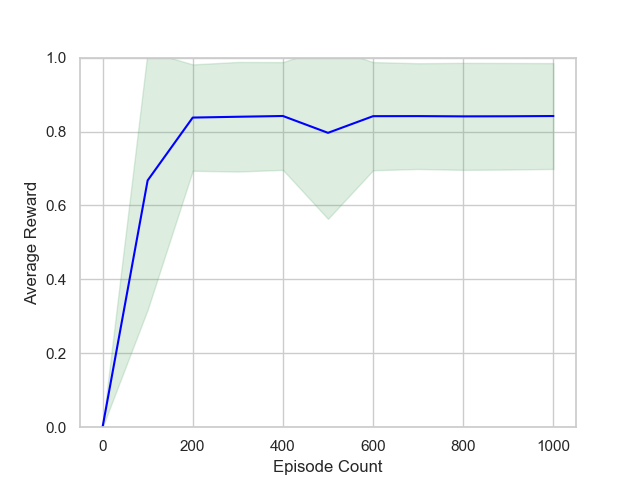
\includegraphics[width=4.5cm]{ep_1000_it_10000_MDP3_gamma_095_re2_ini22_nts_c095_20times.png}
     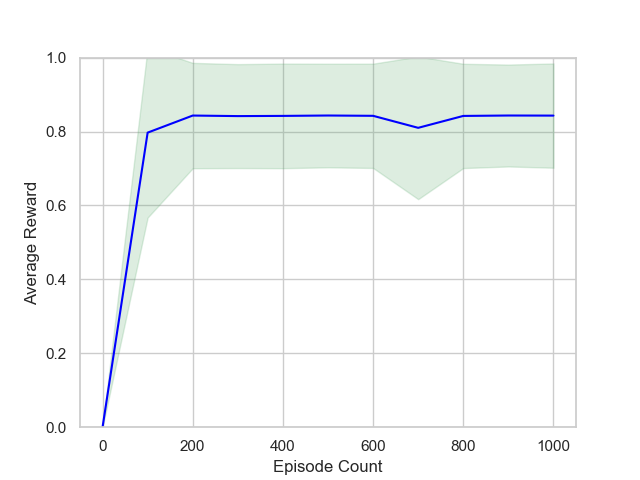
\includegraphics[height = 4.5cm, width=5.5cm]{ep_1000_it_10000_MDP3_gamma_095_re2_ini22_nts_c095_20times_no2.png}
 \end{minipage}

 \begin{minipage}{0.5\hsize}
   \centering
%   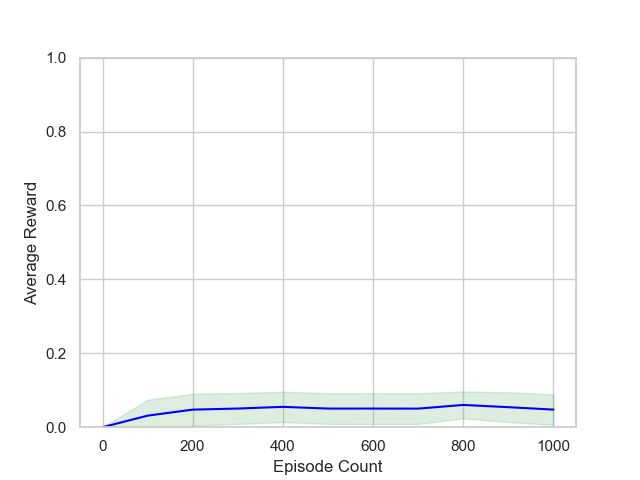
\includegraphics[width=4.5cm]{ep_1000_it_10000_MDP3_gamma_095_nts_c095_abate_20times.png}
   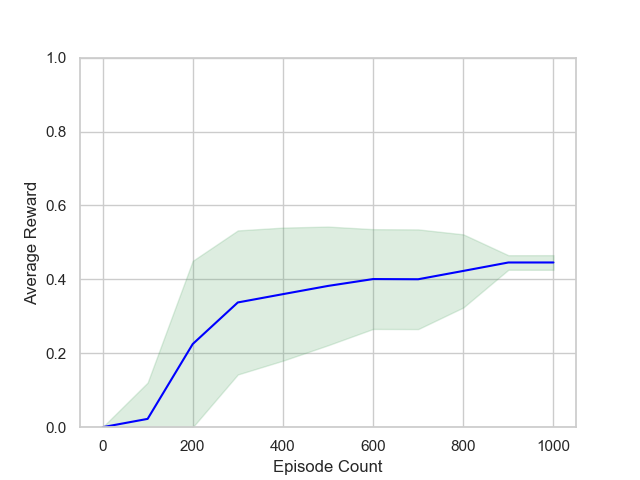
\includegraphics[height = 4.5cm, width=5.5cm]{ep_1000_it_10000_MDP3_gamma_095_nts_c095_ldba_20times.png}
 \end{minipage}
\end{tabular}
 \caption{The arithmetic mean of average reward in each episode for 20 learning sessions obtained from our proposed method (left) and the method using tLDBA (right). They are plotted per 100 episodes and the green areas represent the range of standard deviations. }
 \label{result}
\end{figure}

\begin{figure}[tbp]
 \centering
 \begin{tabular}{c}

   \begin{minipage}{0.52\hsize}
     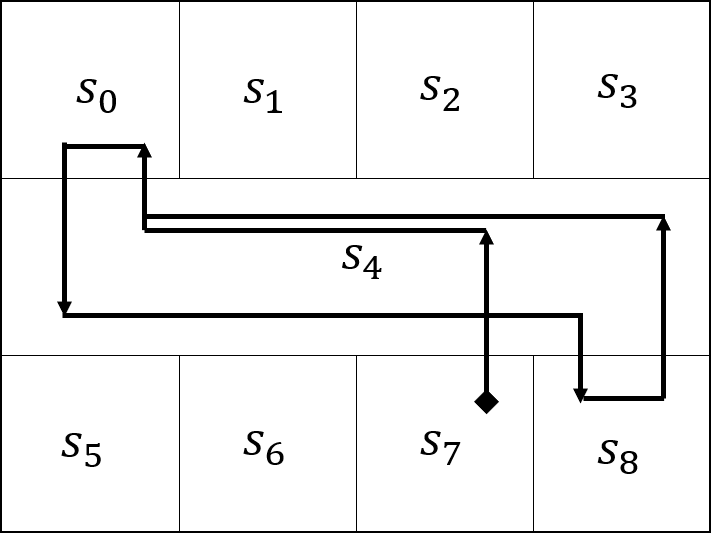
\includegraphics[height = 3.5cm, width=4.5cm]{proposed_policy.png}
   \end{minipage}

   \begin{minipage}{0.52\hsize}
     \centering
     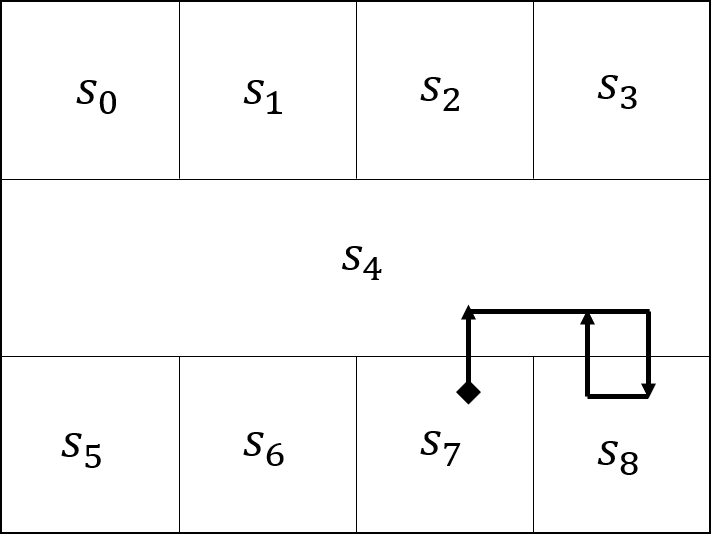
\includegraphics[height = 3.5cm, width=4.5cm]{Abate_policy.png}
   \end{minipage}
 \end{tabular}

 \caption{The optimal policy obtained from our proposed method (left) and the method in \cite{HAK2019, HKAKPL2019} (right).}
 \label{optimal}
\end{figure}
